% Preambuła
\documentclass[a4paper,11pt]{article}
\usepackage[polish]{babel}
\usepackage[OT4]{fontenc}
\usepackage[utf8]{inputenc}
\usepackage{geometry}
\usepackage{fancyhdr}
\usepackage{minted}
\usepackage{graphicx}

\geometry{lmargin=2cm}
\pagestyle{fancy}
\lhead{ZBD - zadanie 2}
\rhead{Piotr Zalas}

% Część główna
\begin{document}

Testy były przeprowadzone przy pomocy skryptów generujących zapytania SQL, które uruchamiałem w ten sposób:

\begin{minted}{bash}
python skrypt.py | ./sqlplus system/manager@//localhost:1521/ORCL > /dev/null
\end{minted}

{\bf Pierwszy test zajętości miejsca} \\

W ramach testu utworzyłem dwukolumnową tabelę. W pierwszej kolumnie znajdowało się
100 tys. identyfikatorów. Każdemu identyfikatorowi była przyporządkowana określona ilość elementów w drugiej kolumnie,
która to ilość była zmienną w trakcie testów. Przeprowadziłem 100 iteracji testu począwszy od wartości 1 z krokiem
równym 10. Mierzone były: rozmiar tabeli i rozmiar indeksów (bez kompresji, ze zwykłą kompresją, z zaawansowaną
kompresją) założonych na pierwszej kolumnie i obydwu kolumnach. Wyniki zapisałem w tabeli, którą następnie eksportowałem. 
Programy testujące umieściłem w plikach miejsce.py (główny skrypt, uruchamiany jak wyżej) i sizetest.sql (na danej tabeli zakłada indeksy, mierzy ich rozmiar i zapisuje wyniki). Zrzut tabeli z wynikami 
umieściłem w pliku wyniki1.txt. Pod koniec testu w tabeli ,,testy'' znajdowało się 10100000 wierszy. Wyniki podsumowałem
na poniższych wykresach:

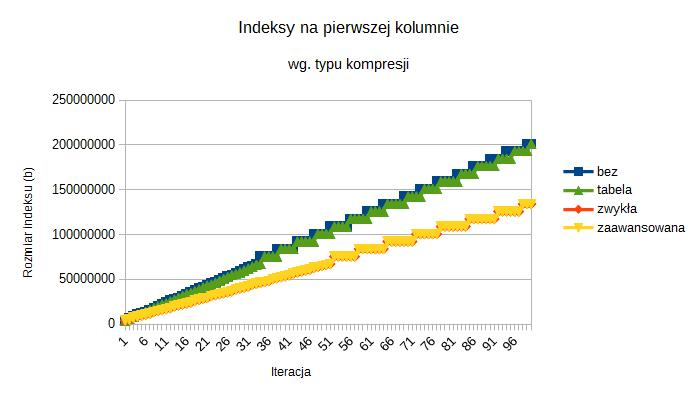
\includegraphics[width=\textwidth]{obr1t.jpg}

Rozmiar indeksu bez kompresji był nieznacznie większy od rozmiaru tabeli. Rozmiar indeksów ze zwykłą kompresją i z
zaawansowaną kompresją był identyczny (najprawdopodobniej dlatego, że były one założone na tylko jednej kolumnie).
Pod względem zajętości miejsca zdecydowanie warto w takiej sytuacji korzystać z kompresji indeksów, zysk w takim
przypadku wynosi ok. 30\%.

Ciekawsze są testy z indeksami założonymi na obydwu kolumnach:

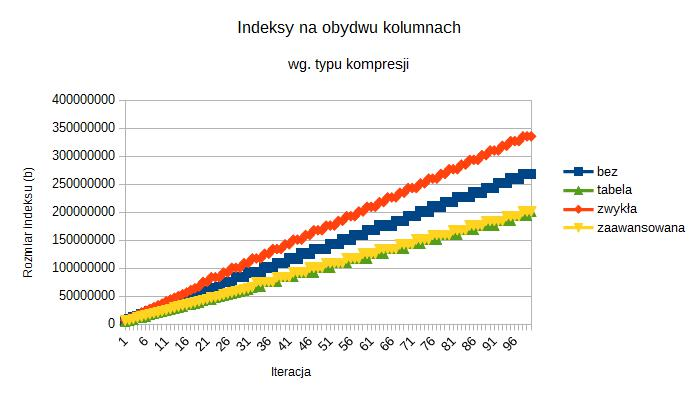
\includegraphics[width=\textwidth]{obr2t.jpg}
Najgorsze okazały się indeksy kompresowane parametrem ,,COMPRESS", które zajęły 25\% więcej miejsca niż
indeksy bez kompresji. Jest to dość zaskakujące, taka sytacja nie powinna mieć miejsca i po lekturze dokumentacji nie przychodzi mi do głowy żadne sensowne wytłumaczenie tego faktu. Zdecydowanie takie rozwiązanie się nie opłaca.
Indeksy z kompresją zaawansowaną (,,COMPRESS ADVANCED LOW") zajęły na dysku nieznacznie więcej miejsca od tabeli. Zysk w porównaniu do zwykłego indeksu wyniósł 25\%. \\

{\bf Testy wydajności i drugi test zajętości miejsca} \\

W tym teście przyjąłem nieco inną strategię generowania tabeli. Tabela testowa ma trzy kolumny, każdy element w pierwszej kolumnie ma przypisane 100 elementów w drugiej, każdy element z drugiej ma przypisanych 100 elementów z trzeciej. Po każdej iteracji testu będę dopisywał $10 \cdot 10^4$ wierszy (generowanych losowo, zgodnie z powyższymi zasadami), co w ostatniej iteracji da 5 milionów wierszy. Maksymalną wartością w kolumnie będzie milion, aby zgodnie z zasadą szufladkową Dirichleta dane mogły się ,,zagęścić''.

W przeciwieństwie do poprzedniego testu, indeks będzie zawsze zakładany na całej tabeli, różnice będą w rodzaju kompresji i wielkości kompresowanego prefiksu (opcja ,,COMPRESS n'', gdzie $n \in {1, 2, 3}$). Oprócz czasu zapytań
zmierzę też wielkość indeksu i tabeli, bez kalkulacji realnego rozmiaru zajętego miejsca. Zazwyczaj bowiem interesuje nas raczej ilość zajętego miejsca na dysku, niźli realna ilość miejsca wykorzystanego na składowanie indeksu.

Będą wykonywane trzy zapytania: zapytanie punktowe, range scan na pierwszej kolumnie, zapytanie o zakres po drugiej kolumnie (skip scan). Ich parametry będą ustalane losowo. Aby uzyskać mierzalny wynik będę zliczał czas wykonania 100000 zapytań. Na wszelki wypadek w zapytaniu umieszczę wskazówkę dla optymalizatora, żeby używał indeksu:

\mint{sql}{
SELECT /*+ INDEX (testy test_ix)*/ ... FROM testy WHERE ...
}

Po wykonaniu testów zrzuciłem wyniki do plików test2\_*.csv. Zobaczmy wykresy:

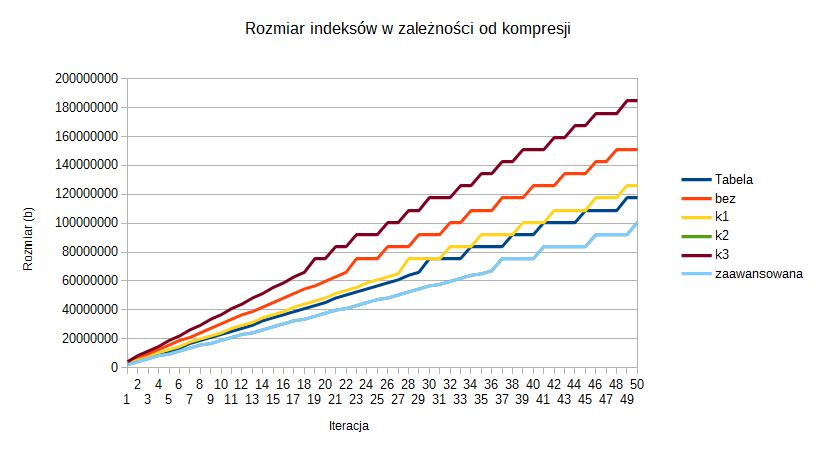
\includegraphics[width=\textwidth]{rozmiar.jpg}

Rozmiar indeksu na dwóch pierwszych kolumnach jest równy rozmiarowi indeksu z zaawansowaną kompresją. Jest to wynik
lepszy od rozmiaru tabeli. Kolejne w kolejności są rozmiary: tabeli, indeksu z kompresją na pierwszej kolumnie,
indeksu bez kompresji, indeksu z kompresją na wszystkich kolumnach. Na wykresach jasno widać, co ile iteracji alokowane były nowe ekstenty i że ich rozmiar wzrastał w dość równomierny sposób.
Na podstawie wykresów można zaryzykować tezę, że opłaca się zakładać kompresowany indeks jeśli kompresowany prefiks
występuje przynajmniej 100 razy w tabeli. Wtedy rozmiar takiego indeksu jest mocno zbliżony do rozmiaru oryginalnej tabeli. Zupełnie nie opłaca się wykonywać kompresji na kolumnach, które złączone dają unikalne wartości w wierszach, nawet jeśli ich prefiksy się powtarzają. Zbieżność wyników otrzymanych dla kompresji zaawansowanej i kompresji na
dwóch kolumnach sugeruje, że algorytm kompresujący w każdym wypełnionym bloku testuje, na ilu kolumnach warto
założyć kompresję i wybiera najbardziej optymalną wartość, po czym stosuje na tak dobranym parametrze zwykłą kompresję. Nie ma tutaj raczej żadnej głębszej filozofii takiej jak
dynamiczny dobór wielkości słownika, wykorzystanie specyficznych własności kompresowanych wartości itd.

Wyniki testów wydajnościowych nie napawają optymizmem:\\
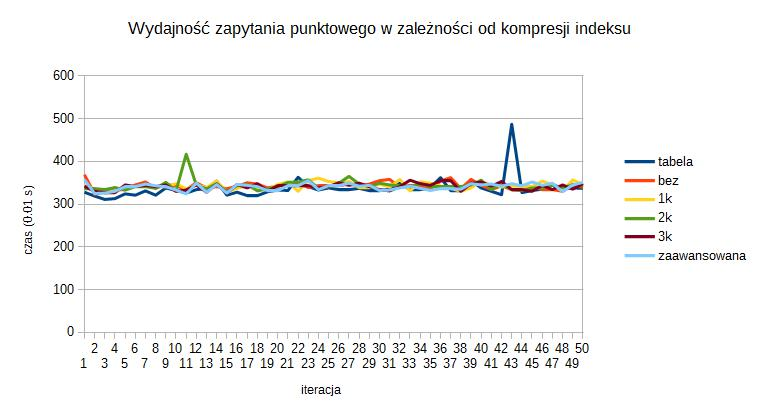
\includegraphics[width=\textwidth]{ta1.jpg}
Tak małe różnice w wydajności zapytań na tabeli zawierającej kilkanaście tysięcy wierszy a tabeli zawierającej 5 milionów wierszy sugeruje, że przy opracowywaniu testu popełniłem jakiś błąd. Aby odzyskać jakiekolwiek wnioski z pomiarów przygotowałem wykres wydajności relatywnej względem zapytania na tabeli bez indeksu:\\
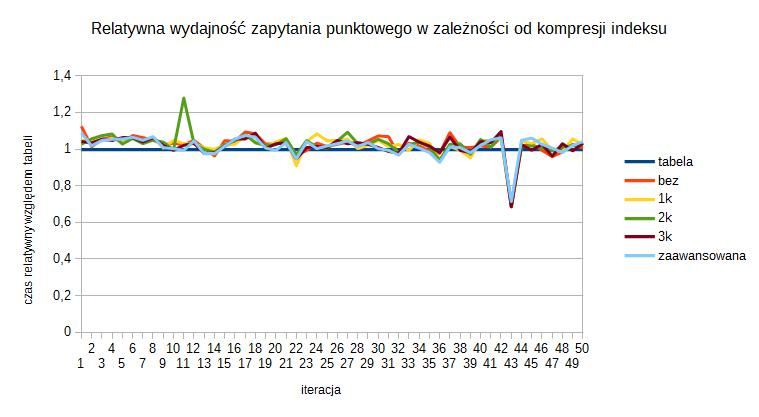
\includegraphics[width=\textwidth]{ta2.jpg}
Jak widać, założenie indeksu powoduje spowolnienie wykonania zapytania o 5 - 10 procent. Wykresy pozostałych zapytań wyglądają analogicznie:\\
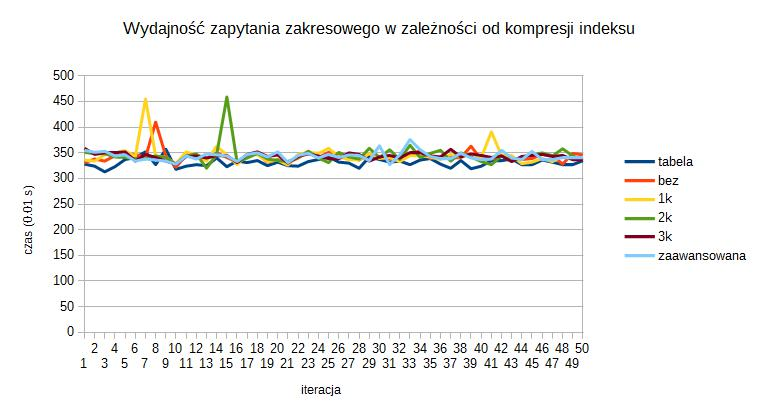
\includegraphics[width=\textwidth]{tb1.jpg}
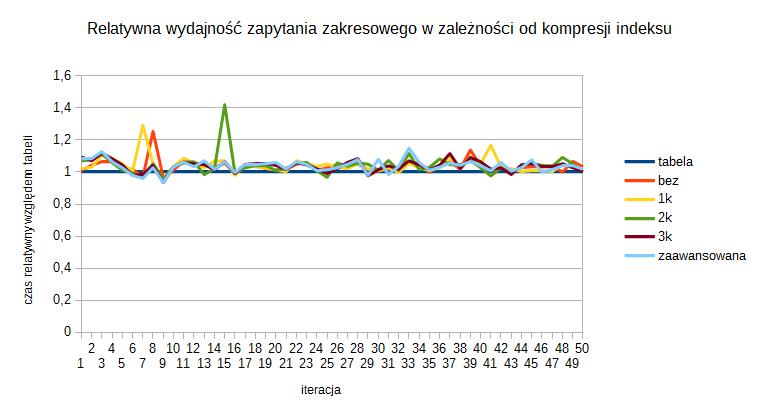
\includegraphics[width=\textwidth]{tb2.jpg}
Nawet czasy wykonania są podobne. Powstaje tutaj pytanie, jaki błąd został popełniony przy przygotowywaniu testu?
Czy jest to skutek zbyt małego zbioru testowego, a może błędu w skryptach? Prawdopodobnie tabela testowa była na
tyle mała, że mieściła się w całości w pamięci operacyjnej. W tym momencie zysk dawany przez indeksy znikał i nawet
full scan na tabeli działał w sensownym czasie. Pozostaje tutaj otwarte pytanie, dlaczego nawet w zapytaniu punktowym indeks bez kompresji był wolniejszy od operacji na tabeli bez indeksu. W przypadku błędu w skryptach najbardziej 
prawdopodobnym winowajcą jest funkcja open na kursorze, która być może nie czeka na wyliczenie całego wyniku (chociaż w dokumentacji jest sugestia, że tak nie powinno być). Zamiast wykonać chociaż jednego fetcha natychmiast zamykałem kursor, co mogło anulować wykonanie zapytania. Za tą hipotezą przemawiają łudząco podobne czasy zapytań na wszystkich wykresach niezależnie od rozmiaru tabeli.\\
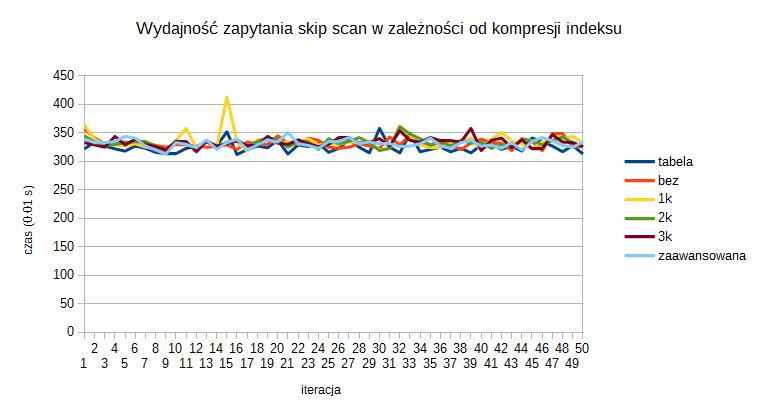
\includegraphics[width=\textwidth]{tc1.jpg}
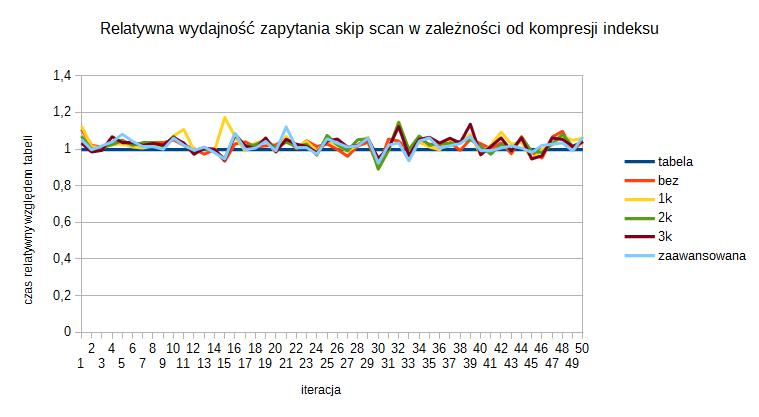
\includegraphics[width=\textwidth]{tc2.jpg}
Podsumowując, jeśli pomiary były poprawne to nie opłaca się tutaj zakładać indeksów.
\end{document}

